% !TeX root = ../../paper.tex
\subsection{Mini-Max-Suche}

Im Schachspiel ist jeder Spieler bestrebt, das für ihn bestmögliche Spielergebnis zu erzielen.
Zur Abbildung dieses Prinzips dient der \textit{Mini-Max}-Algorithmus [\cite{Russell2010}].
Um dies abbilden zu können wird ein Punktwert eingeführt, den ein Spieler zu maximieren versucht und der andere Spiele zu minimieren versucht.
Für das Schachspiel und die spätere Betrachtung dessen wird an dieser Stelle festgelegt, dass eine hohe Bewertungen für einen Vorteil der weißen Spielseite steht, wohingegen eine negative Bewertungen für einen Vorteil für die schwarze Spielseite steht.
Somit ist Weiß bestrebt, den Wert durch die Wahl einer Spieloption zu maximieren und Schwarz den Wert zu minimieren [\cite{Paulsen2009}].
Zur Berechnung dieses Punktwertes wird ein Spielbaum (engl. \textit{game tree}) benötigt, der alle möglichen Spielzüge beinhaltet.
Es werden alle Knoten eines Spielbaumes mit ihren zugehörigen Werten generiert [\cite{Shah2007}].
Die Knoten innerhalb des Baumes werden in drei verschiedene Kategorien unterteilt: Blattknoten, minierende und maximierende Knoten.
Jeder Blattknoten erhält seinen Nutzwert (engl. \textit{utility value}).
Den minimierenden Knoten wird jeweils der kleinste Wert ihrer Kindknoten zugewiesen, den maximierenden Knoten jeweils der größte Wert [\cite{Shah2007}].
Abbildung~\ref{fig:minimax_tic-tac-toe} zeigt einen Teil eines Spielbaums für das Spiel Tic-Tac-Toe, der die einzelnen Schritte der Berechnung durch den Mini-Max-Algorithmus beinhaltet.

\begin{figure}
    \centering
    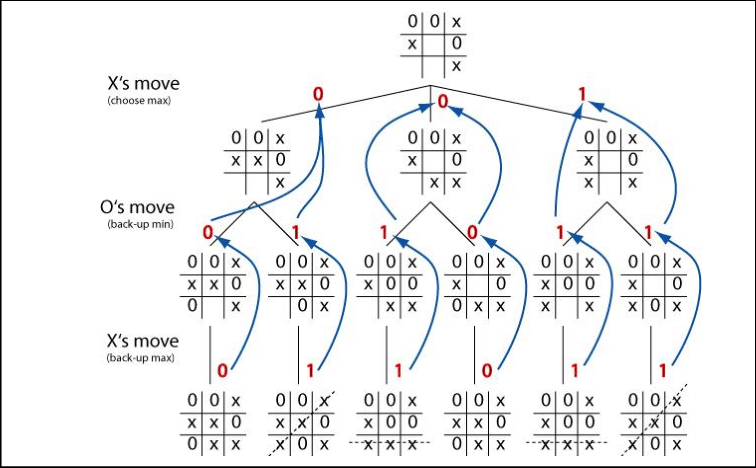
\includegraphics[width=0.89\textwidth]{images/theory/minimax_tic-tac-toe.png}
    \caption[Spielbaum eines Tic-Tac-Toe Spiels erstellt mittels des Mini-Max-Algorithmuses]{Spielbaum eines Tic-Tac-Toe Spiels erstellt mittels des Mini-Max-Algorithmuses [\cite{Elnaggar2014}]}
    \label{fig:minimax_tic-tac-toe}
\end{figure}

Die Ausgangssituation des Spiel ist an der Wurzel des Baumes abgebildet.
Im Falle des Spiels Tic-Tac-Toe wird festgelegt, dass Spieler X bestrebt ist, den Punktwert zu maximieren, wohingegen Spieler O bestrebt ist, diesen zu minimieren.
Spieler X ist als nächstes am Zug und besitzt drei Möglichkeiten, sein Kreuz auf dem Spielfeld zu platzieren.
Dem folgt der Spielzug des Spielers O, der seinerseits für jeden möglichen Spielzug von Spieler X je zwei Möglichkeiten besitzt, sein Symbol zu setzen.
Somit gibt es von der Ausgangslage her sechs mögliche Spielzüge, die Spieler O durchführen kann.
Zu guter Letzt hat Spieler X für jede seiner Ausgangslagen nur noch eine Möglichkeit, sein Kreuz zu setzen.
Jeder mögliche Endstand des Spiels erhält nun einen Punktwert.
Markiert der Endstand einen Sieg für Spieler X, so erhält dieser den Wert 1, bei einem Sieg für Spieler O den Wert -1 und bei einem Unendschieden den Wert 0.
Die Werte der Blattknoten werden anschließend nach oben propagiert.
Maximierende Knoten (Spieler X ist am Zug) übernehmen den jeweils höchsten Zahlenwert, minimierende Knoten (Spieler O ist am Zug) den niedrigsten Wert.
Am Ende dieses Prozesses ist von der Ausgangslage des Spiels erkennbar, dass Spieler X dem rechten Pfad des Baumes folgen muss, um garantiert einen Sieg zu erzielen, es für ihn aber auch bei einer Fehlentscheidung im nächsten Zug noch möglich ist, das Spiel zu gewinnen.
Beim Schach ist es jedoch in der Regel nicht möglich alle Positionen bis zum Spielende zu analysieren.
Im Gegenteil zu Tic-Tac-Toe, bei dem der Spielbaum maximal die Tiefe neun erreicht, kann beim Schach theoretisch eine Tiefe von 5899 erreicht werden [\cite{Wikipedia2018}].
Da es im Verlauf eines Schachspiels durchschnittlich $x$ mögliche Züge für den Spieler am Zug gibt, gibt es ab einer bestimmten Tiefe $t$, $x^t$ zu analysierenden Positionen.
Weil sogar schnelle Computer bei diesem exponentiell wachsenden Baum zu hohe Rechenzeiten benötigen, muss eine maximale Tiefe, bis zu der der Spielbaum analysiert wird, festgelegt werden.
Diese ist je nach Anspruch bei präzisen Evaluationen tiefer, bei schnellen Evaluationen weniger tief.
Um den Minimax Algorithmus auf Programmierebene umzusetzen, werden folgende Methoden benötigt [\cite{Shannon1950}]:

\begin{itemize}
    \item Sammelt für eine Position die erlaubten Züge. Hierfür muss sowohl auf verschiedenen Zugarten der Figuren und Schach eingegangen werden, als auch Sonderzüge wie En-Passant und die Rochade berücksichtigt werden.
    \item Die Kernaufgabe des Minimax Algorithmus umsetzt, also das abwechselnde Maximieren und Minimieren der möglichen Folgezüge einer Position.
    \item Die statische Eval-Function aus Kapitel 2.1 umsetzt.
    \item Kann für eine Position Schachzüge ausführen und diese auch rückgängig machen
\end{itemize}

Bei der Umsetzung der Kernaufgabe des Minimax-Algorithmus wird der Ansatz von [\cite{Knuth1975}] übernommen.
Außerdem wird die Standard-Implementierung verwendet, bei der der gesamte Algorithmus in zwei Prozeduren, Minimize und  Maximize, aufgeteilt wird.
Diese führen dabei jene Tätigkeiten aus, welche die Entscheidungen des minimierenden bzw. maximierenden Spielers repräsentieren.
Bei der alternativen Negamax-Implementierung gibt es nur eine Minimax-Prozedur welche die Funktionen beider Spieler übernimmt [\cite{Wikipedia2020}].
Ist ein Spielbaum gegeben, so lässt sich die optimale Strategie basierend auf den Minimax-Werten (engl. \textit{minimax values}) der einzelnen Knoten ableiten.
Diese optimale Strategie wird als $\text{MINIMAX}(n)$ geschrieben und ist in Formel~\ref{eq:minimax_general-function} dargestellt [\cite{Russell2010}].

\begin{equation} \label{eq:minimax_general-function}
    \text{MINIMAX}(s) =
    \begin{cases}
        \text{UTILITY}(s) \hfill \text{*} \\
        max_{a \in Actions(s)} \text{MINIMAX}(\text{RESULT}(s, a)) \hfill \text{**} \\
        min_{a \in Actions(s)} \text{MINIMAX}(\text{RESULT}(s, a)) \hfill \text{***} \\
    \end{cases}
\end{equation}

\begin{align*}
    \begin{split}
        & \text{*\ \ \ \ if TERMINAL-TEST}(s) \\
        & \text{**\ \ \ if PLAYER(s)} = \text{MAX} \\
        & \text{***\ \ if PLAYER(s)} = \text{MIN}
    \end{split}
\end{align*}

Dabei gelten folgende Aussagen [\cite{Russell2010}]:

\begin{itemize}
    \item $s$ ist der aktuelle Zustand bzw. Knoten im Spielbaum.
    \item $a$ ist eine Aktion bzw. ein Halbzug.
    \item Die Funktion $\text{UTILITY}$ gibt den Nutzwert für einen Blattknoten zurück.
    \item Die Funktion $\text{PLAYER}$ gibt den Spieler zurück, der am Zug ist ($\text{MAX}$ für Weiß und $\text{MIN}$ für Schwarz).
    \item Die Funktion $\text{Actions}$ liefert die Menge der für den übergebenen Zustand gültigen Züge.
    \item $\text{TERMINAL-TEST}$ gibt den Wert $true$ zurück, wenn das Spiel zu Ende (erreichen eines Blattknotens), ansonsten $false$.
    \item $\text{RESULT}$ liefert den Zustand zurück, der folgt, wenn auf den Zustand $s$ die Aktion $a$ angewandt wird.
\end{itemize}

Für den Minimax-Wert, den die Funktion $\text{MINIMAX}$ liefert, wird angenommen, dass beide Spieler bis zum Ende des Spiels optimal spielen [\cite{Russell2010}].
Da der Minimax-Algorithmus in dieser Form sehr rechenintensiv ist und viel Speicher benötigt, wird er durch eine maximale Tiefe begrenzt (\textit{begrenzte Tiefensuche}).
Zur Umsetzung dieser begrenzten Tiefensuche werden Funktionen $F$ (Formel~\ref{eq:minimax_white-players-function-with-depth}) für den Spieler Weiß und $G$ (Formel~\ref{eq:minimax_black-players-function-with-depth}) für Spieler Schwarz definiert.
Die beiden Funktionen definieren das Verhalten der Spieler beim Treffen auf eine Schachposition $p$ in der Tiefe $t$.

\begin{equation} \label{eq:minimax_white-players-function-with-depth}
    F(p, t) =
    \begin{cases}
        e(p) \quad \text{if } t = 0,\\
        max(G(p_1, t - 1), G(p_2, t - 1), ... , G(p_l, t - 1)) \quad \text{if } t > 0
    \end{cases}
\end{equation}

\begin{equation} \label{eq:minimax_black-players-function-with-depth}
    G(p, t) =
    \begin{cases}
        e(p) \quad \text{if } t = 0,\\
        min(F(p_1, t - 1), F(p_2, t - 1), ... , F(p_l, t - 1)) \quad \text{if } t > 0
    \end{cases}
\end{equation}

Dabei sind $p_1$, ... , $p_l$ die möglichen Positionen, welche nach einem Zug aus der Position p resultieren können und $e(p)$ die Bewertungsfunktion ist.
Der Pseudocode für einen Minimax mit Tiefenbegrenzung ist in Algorithmus~\ref{alg:minimax_minimax-with-depth} dargestellt.
Die verwendeten Hilfsfunktionen $p.move(m)$ und $p.undoMove(m)$ führen auf der Schachstellung $p$ den Zug $m$ aus, beziehungsweise machen ihn rückgängig.
Es kann, anders als bei der Negamax-Implementierung, dieselbe Bewertungsfunktion für beide Funktionen benutzt werden, weil diese weiß-favorisierende Positionen mit positiven Werten und schwarz-favorisierende Positionen mit negativen Werten bewertet.
Die Zahl $d$ repräsentiert die Tiefe (engl. \textit{depth}), $evaluate$ ist die Bewertungsfunktion und die Hilfsfunktion $findLegalMoves(p)$ gibt die Menge der zulässigen Halbzüge für $p$ zurück.
Der Punktwert (engl. \textit{score}) wird in der Variablen $score$ gespeichert.

\begin{algorithm}[H]
    \caption{Minimax mit Tiefenbegrenzung}
    \label{alg:minimax_minimax-with-depth}
    \begin{algorithmic}[1]
        \Function{maximize}{Integer $d$, Position $p$}
        \If{$d < 1$}
        \State \Return evaluate($p$)
        \Else
        \State $score \gets -\infty$
        \State $legalMoves \gets findLegalMoves(p)$
        \ForAll {$m$ in $legalMoves$}
        \State p.move(m)
        \State $moveScore \gets minimize(d-1, p)$
        \State p.undoMove(m)
        \If{$moveScore > score$}
        \State $score \gets moveScore$
        \EndIf
        \EndFor
        \EndIf
        \State \Return $score$
        \EndFunction
        \Function{minimize}{Integer $d$, Position $p$}
        \If{$d < 1$}
        \State \Return evaluate($p$)
        \Else
        \State $score \gets \infty$
        \State $legalMoves \gets findLegalMoves(p)$
        \ForAll {$m$ in $legalMoves$}
        \State p.move(m)
        \State $moveScore \gets maximize(d-1, p)$
        \State p.undoMove(m)
        \If{$moveScore < score$}
        \State $score \gets moveScore$
        \EndIf
        \EndFor
        \EndIf
        \State \Return $score$
        \EndFunction
    \end{algorithmic}
\end{algorithm}
